\documentclass{beamer}

\usepackage[ngerman]{babel}
\usepackage[T1]{fontenc}
\usepackage{graphicx}
\usepackage{verbatim}
\usepackage{mdwlist}
\usepackage{listings}
\usepackage{ragged2e}

\usepackage{xunicode}
\usepackage{xltxtra}
\defaultfontfeatures{Mapping=tex-text}
\setmonofont[Mapping={}, Scale=MatchLowercase]{DejaVu Sans Mono}
\setsansfont[Scale=MatchLowercase]{Linux Biolinum O}
\setmainfont[]{Linux Libertine O}

\newbox\mytempbox
\newdimen\mytempdimen
\newcommand\includegraphicscopyright[3][]{%
  \leavevmode\vbox{\vskip3pt\raggedright\setbox\mytempbox=\hbox{%
  \includegraphics[#1]{#2}}%
    \mytempdimen=\wd\mytempbox\box\mytempbox\par\vskip1pt%
    \fontsize{3}{3.5}\selectfont{\color{black!25}{\vbox{\hsize=\mytempdimen#3}}}\vskip3pt%
}}

\let\raggedright=\RaggedRight
\hyphenation{Freeze}

\newcommand\prelim[1]{\small }

\newcommand\strColor[1]{\color{beamer@blendedblue}{#1}}

\newcommand\sect[1]{\begin{center}\huge\strColor{#1}\end{center}}

\setbeamerfont{page number in head/foot}{size=\large}
\setbeamertemplate{navigation symbols}{}
\setbeamertemplate{headline}
{%
    \begin{beamercolorbox}{section in head/foot}
        \vskip1em
        \insertsection\hfill
\includegraphics[height=5em]{FULogo_RGB.eps}\hspace{1em}
        \vskip-5.3em
    \end{beamercolorbox}%
}
\setbeamertemplate{footline}[frame number]

\title{OParl-Validator}
\author{Das OParl-Validator-Team}
\institute{Freie Universität Berlin\\Institut für Informatik}
\date{$n$. Oktober 2014}

\begin{document}

\frame{\titlepage}

%\frame{\tableofcontents}

\frame{
    \frametitle{Gliederung}
    \begin{itemize}
        \item Organisation
        \item Architektur
        \item Features
        \item Close-Out-Plan
        \item Demo
    \end{itemize}
}

\frame{
    \frametitle{Organisation}
    \begin{itemize}[<+->]
        \item Prozesse
        \begin{itemize}
            \item Kanban auf Trello
            \item Continuous Integration
        \end{itemize}
        \item Meetings
        \begin{itemize}
            \item Mumble und Hangout
            \item Häufig mit Stakeholdern
        \end{itemize}
        \item Hackathons bei Spline
        \item Protokolle
    \end{itemize}
    
    
 


}

\frame{
    \frametitle{Organisationsprobleme und -lösungen}
}

\frame{
    \frametitle{Features}
    \begin{itemize}[<+->]
        \item Continuous Integration
        \begin{itemize}[<*>]
            \item Dank Travis CI
            \item Mit automatischer Coverage dank Coveralls
        \end{itemize}
        \item Python 2.7 und 3.3
        \begin{itemize}[<*>]
            \item \texttt{six}-Library sehr hilfreich
            \item Continuous Integration ebenso
        \end{itemize}
        \item Back-off Modi
        \begin{itemize}[<*>]
            \item Was meinte ich denn hiermit?
        \end{itemize}
        \item Constraints
        \begin{itemize}[<*>]
            \item Type Whitelist, Rekursion, etc.
        \end{itemize}
    \end{itemize}
}

\frame{
    \frametitle{Featureprobleme und -lösungen}
}

\frame{
    \frametitle{Demo}
    Slide mit Absicht leer – mit Ausnahme der Überschrift, des FU-Logos, des Foliums und dieses Textes
}

\frame{
    \frametitle{Architektur}
    \begin{columns}
        \begin{column}{.5\textwidth}
            \begin{itemize}[<+->]
                \item Validator
                \begin{itemize}[<*>]
                    \item Basierend auf Freeze vom 22. Juli
                    \item Mit einigen optionalen Features
                \end{itemize}
                \item Crawler
                \begin{itemize}[<*>]
                    \item Validiert ein komplettes System
                    \item Oder einen Teil des Systems
                \end{itemize}
                \item Server-Tests
                \begin{itemize}[<*>]
                    \item Suite mit Anforderungen auf tieferer Abstraktionsebene
                    \item Aber auf Layer 7
                \end{itemize}
                \item Command Line Interface
                \begin{itemize}[<*>]
                    \item Gemeinsamer Entry-Point
                \end{itemize}
            \end{itemize}
        \end{column}
        \begin{column}{.5\textwidth}
            \vspace{-.5cm}
            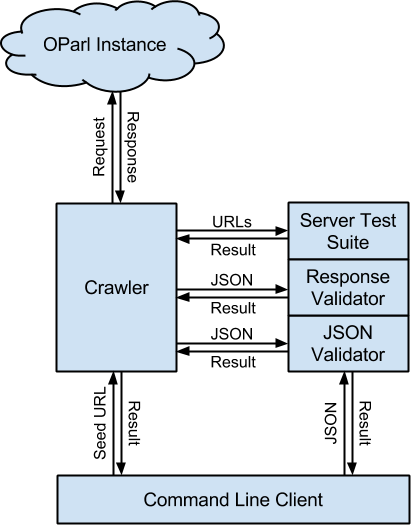
\includegraphics[width=\textwidth]{architecture.final.png}
        \end{column}
    \end{columns}
}

\frame{
    \frametitle{Architekturprobleme und -lösungen}
    \begin{itemize}[<+->]
        \item JSON- vs. Dict-Validierung
        \begin{itemize}[<*>]
            \item Dict: Vereinfacht den Code im Validator
            \item \textbf{JSON}: Erlaubt zentrale Behandlung von Fehlern im Validator
        \end{itemize}
        \item Server-Tests
        \begin{itemize}[<*>]
            \item Parallel: Beste Abdeckung aber unzählige Requests
            \item \textbf{Final}: Schneller, flexibler, aber erfordert Sammlung der URLs
        \end{itemize}
        \item Paralleles oder finales Reporting
        \begin{itemize}[<*>]
            \item Parallel: Der Benutzer kann abbrechen und bereits gefundene Fehler beheben
            \item \textbf{Final}: Spart ein paar Zeilen Code
        \end{itemize}
    \end{itemize}
}

\frame{
    \frametitle{Close-Out-Plan}
    \begin{itemize}[<+->]
        \item OParl 1.0 noch nicht finalisiert
        \item Einige des Teams werden die letzten Anpassungen zu gegebener Zeit vornehmen
        \item Einige des Teams werden das Projekt auch langfristig zusammen warten
    \end{itemize}
}
\end{document}
   Organisation: 



1. Unsere Kunden:

- direkt: OParl Entwickler(Kontakt: Marian(hauptsächlich: fusepool finanziert eu projekt; aus Köln; Lucas hat ihn getroffen),
Community:  Andreas(semantic-web-consultant), Stefan )
Viel Kommunikation war wichtig und richtig, da viele Änderungen und Diskussionen in/wegen der Spezifikation aufkamen


- indirekt:  RIS Hersteller wie CC e-Gov GmbH , PROVOX Systemplanung GmbH ,QuinScape GmbH , Somacos GmbH und Co. KG,Sternberg Software-Technik GmbH ,  sowie zukünftige Projekte, welche den OParl verwenden wollen--> Nutzer . 

2. Unsere Arbeitsweise:
- Kein Vertrag freies miteinander Arbeiten !
- Regelmäßige Treffen Mittwochs, bei denen auch die Kunden mittels Telefon eingebunden werden und eine regelmäßige Telefonkonferenz am Freitag auch größere Runde : Auch Oparl generell! 
- Kanban Prinzip
- Außerdem herrscht Kommunikation mit Hilfe einer Mailingliste
- Aufgaben werden nach Fähigkeiten und Dringlichkeit gewählt(Kanban)
- Hack-a-thons bei Spline
- Protokollieren der Treffen

3. Unsere Milestones: Fazit

3.1.
3.2. Web-Frontend nicht so wichtig! 
3.3.
3.4. JSON-LD wird nicht komplett unterstützt!
3.5.

4. Softwaretechnische Methoden und Informatische Techniken.

4.1 Wie geplant wurde zur Realisierung des Kanban Prinzips Trello verwendet
4.2 Das test-driven-development für die Library angwendet; keine Webanwendung
4.3 Es wurde ein GitHub Repository eingerichtet. Später wechselten wir ins offizelle OParl
4.4 Wie geplant viel mit JSON-Schema erfüllt. Den Rest mit Hilfe von individuellen Test
4.5 bereits „genommene“ Pfade werden vom Crawler nicht erneut „genommen“.
4.6 Wird nun schlicht und funktional gehalten. Soll auch speezielle Tests durchführen können um Zeit zu Sparen

5. Rollen:

5.1 Wie geplant hat Lucas den Kontakt mit unseren Kunden gehalten und die Meetings mit ihnen Organisiert.
5.2 Telofy konnte uns mit seiner Rolle als Python- Supporter vieles beitragen.
6. Sprachen, Frameworks und Werkezeuge
6.1 Buidlout und JSON-Schema haben sich als sehr hilfreiche tools herausgestellt.
6.2 Durch die Verwendung von Flask wird auf einfachem Weg das Web-frontend erstellt.
6.3 Wie geplant haben wir Python 2.7 und Python 3.0 unterstützt
7. Risikomanagement:
7.1 viele Änderungen in der Spezifikation, auch noch nach dem eigentlichen Versionsfreeze. 
→ Verzögerungen Problem: OParl 1.0 wurde später als geplant erreicht
7.2  Kommunikation mit Kunden funktionierte

8. Benotung:
 Zur Benotung soll nun ein Gesamtbericht von allen Teilnehmern des Projekts erstellt werden, welcher den Verlauf der Entwicklung, sowie die auftretenden Probleme, erläutert. Außerdem wird von jedem Projektteilnehmer ein individueller Tätigkeitsbericht in Stichpunkte
Abschließendes Meeting mit den Wissenschaftlichen Mitarbeitern. 


